% !TEX root = gr20.tex
\documentclass[11pt]{article}
\usepackage[margin=1.1in]{geometry}
\usepackage{amsmath,amssymb,amsthm,mathtools}
\usepackage[T1]{fontenc}
\usepackage{microtype}
\usepackage{booktabs}
\usepackage{graphicx}
\usepackage{xcolor}
\usepackage{algorithm}
\usepackage{algpseudocode}
\usepackage{enumitem}
\usepackage[colorlinks=true,linkcolor=black,citecolor=black,urlcolor=black]{hyperref}

\newcommand{\R}{\mathbb R}
\newcommand{\E}{\mathbb E}
\newcommand{\Q}{\mathbb Q}
\newcommand{\PP}{\mathbb P}
\newcommand{\dd}{\mathrm d}
\newcommand{\dlv}{\Sigma}
\newcommand{\abs}[1]{\lvert #1\rvert}
\newcommand{\ip}[2]{\langle #1,#2\rangle}
\newcommand{\one}{\mathbf 1}
\newcommand{\Var}{\operatorname{Var}}
\newcommand{\Gh}{\widehat G}
\newcommand{\Nh}{\widehat N}
\newcommand{\removeblock}[1]{}
\newcommand{\MW}[1]{{\color{red}#1}}
\DeclareMathOperator{\diag}{diag}
\DeclareMathOperator{\tr}{tr}

\theoremstyle{plain}
\newtheorem{theorem}{Theorem}[section]
\newtheorem{proposition}[theorem]{Proposition}
\newtheorem{lemma}[theorem]{Lemma}
\newtheorem{corollary}[theorem]{Corollary}
\theoremstyle{definition}
\newtheorem{assumption}[theorem]{Assumption}
\theoremstyle{remark}
\newtheorem{remark}[theorem]{Remark}

\title{%
  \textbf{GROMM goes Production}\\[6pt]
  \large Generative Risk-neutral Option Market Models II - Production Grade
}

\author{Hans Buehler$^{*}$\qquad Blanka Horvath$^{*,\#}$\qquad Magnus Wiese$^{*}$\\[0.6em]
  {\small $^{*}$Mathematical Institute, University of Oxford,
  $^{\#}$Oxford-Man Institute, University of Oxford}}
\date{\today}

\begin{document}
\maketitle

\begin{abstract}
   We refine the GROMM model presented in~\cite{GROMM2026} such that it has an expanding strike and expory grid, and
   its parameters can be estimated based on prevailing grid geometry. We compare LSTM and compact Mamba-style selective
   state-space backbones for its discrete local-volatility factor law, including variants with state-dependent spot--volatility
   correlation.

   The resulting model has a near-perfect
   fit to observed option prices and outperforms comparable models in $\PP$-measure simulations.

   [need to decide what else to put in here]
\end{abstract}

\tableofcontents


\section{Introduction}\label{sec:intro}

\section{Factor-Law Evaluation and Portfolio-Conditional Entropic Hedging}
\label{sec:factor-law-and-hedging}

\subsection{Small-sample predictive evaluation}
\label{sec:factor-law-evaluation}

The historical sample is too short to justify selecting a conditional
factor law from its in-sample fit.  We therefore use a rolling-origin
experiment.  The experiment contains four consecutive test blocks of 63
business days, for a total of 252 out-of-fold observations from 13 August
2024 to 28 August 2025.  Before each block, a model is fitted using only
earlier observations.  The number of recurrent training epochs is selected
on the final 20\% of that earlier sample, after which the model is refitted
on the entire pre-block history.

Let $Z_t\in\R^F$ denote the observed factor innovation on day $t$, and let
$C_{m,t}$ be the conditional covariance forecast by model $m$.  The primary
$\Q$-measure diagnostic is the Gaussian negative log score per factor and day,
\begin{equation}
  L^\Q_{m,t}
  :=
  \frac{1}{2F}\left(
    \log\det C_{m,t}
    +Z_t^\top C_{m,t}^{-1}Z_t
  \right).
  \label{eq:q-factor-log-score}
\end{equation}
This is a proper scoring rule for a zero-mean conditional Gaussian factor
law.  The original models use diagonal
$C_{m,t}=\operatorname{diag}(s_{m,t,1}^2,\ldots,s_{m,t,F}^2)$.  To test
state-dependent spot--volatility correlation without estimating an
unrestricted loading matrix, we also fit
\begin{equation}
  C_{m,t}=D_{m,t}
  \begin{pmatrix}1&\rho_{m,t}^\top\\ \rho_{m,t}&I\end{pmatrix}
  D_{m,t},
  \qquad
  \rho_{m,t}
  =\bar\rho\frac{u_{m,t}}{\sqrt{1+\lVert u_{m,t}\rVert_2^2}},
  \qquad \bar\rho=0.95,
  \label{eq:conditional-spot-factor-correlation}
\end{equation}
where the first factor is the Gaussianized spot shock and the remaining
factors are its unconditionally orthogonal DLV residuals.  Hence
$\lVert\rho_{m,t}\rVert_2<\bar\rho$ and the covariance is positive definite
by construction.  Through the fixed DLV loading basis, changing
$\rho_{m,t}$ changes both node-level spot--DLV correlations and the effective
conditional loading directions.

Performance is reported relative to the AR(1) benchmark as the paired daily
improvement
\begin{equation}
  \Delta_m^\Q
  :=
  \frac{1}{T}\sum_{t=1}^T
  \left(L^\Q_{\mathrm{AR}(1),t}-L^\Q_{m,t}\right).
  \label{eq:q-factor-skill}
\end{equation}
Thus, positive values indicate an improvement over AR(1).  Confidence
intervals resample complete days using a moving-block bootstrap with
ten-business-day blocks and 20,000 replications.  The conclusions below are
unchanged with block lengths of five or twenty business days.

For the physical drift, let $b^\PP_{t,f}$ denote the estimated coefficient
of the attainable $\PP$-drift in factor direction $f$, let
$\widehat b^\PP_{m,t,f}$ be its forecast, and let $\tau_f$ be its training
sample standard deviation.  We report
\begin{equation}
  L^\PP_{m,t}
  :=
  \frac{1}{F}\sum_{f=1}^F
  \left(
    \frac{b^\PP_{t,f}-\widehat b^\PP_{m,t,f}}{\tau_f}
  \right)^2.
  \label{eq:p-drift-target-score}
\end{equation}
Unlike~\eqref{eq:q-factor-log-score}, this evaluates an estimated attainable
drift target.  It is not a realized hedging profit-and-loss statistic.

\subsubsection{LSTM and Mamba-style selective state-space factor laws}

Both recurrent models receive the same causal input $x_t$: the standardized
current DLV-level coordinates concatenated with the previous day's factor
innovation.  The latter is set to zero whenever the historical panel is not
contiguous.  From a common hidden state, the output layer predicts the $F$
attainable $\PP$-drift coefficients and the $F$ conditional log-scales.  The
correlated variants additionally predict the $F-1$ unconstrained coordinates
$u_t$ in~\eqref{eq:conditional-spot-factor-correlation}.  Thus the models
differ only in their state update, not in their information set or output
parameterization.

For the LSTM, with $\sigma$ denoting the logistic function, we use
\begin{align}
  (i_t,f_t,g_t,o_t)
    &=\bigl(\sigma,\sigma,\tanh,\sigma\bigr)
      \left(W_xx_t+W_hh_{t-1}+b\right), \\
  c_t&=f_t\odot c_{t-1}+i_t\odot g_t, \\
  h_t&=o_t\odot\tanh(c_t),
  \qquad y_t=W_oh_t+b_o.
  \label{eq:lstm-factor-law}
\end{align}
The hidden and cell states are reset at a break in the daily sequence.

The model denoted ``Mamba'' in the experiments is a compact Mamba-style
selective state-space recurrence rather than a full stacked Mamba3 network.
Its input-dependent retention gate and candidate state are
\begin{align}
  a_t&=\sigma(W_ax_t+b_a),
  &\widetilde h_t&=\tanh(W_cx_t+b_c), \\
  h_t&=a_t\odot h_{t-1}+(1-a_t)\odot\widetilde h_t,
  &y_t&=W_oh_t+b_o.
  \label{eq:selective-ssm-factor-law}
\end{align}
This has fewer recurrent interactions than the LSTM and provides a useful
small-sample test of whether input-dependent memory is sufficient.  Both
models use 32 hidden coordinates.  Their output vector is partitioned as
\begin{equation}
  y_t=
  \left(
    \widehat b_t^\PP,
    \ell_t,
    u_t
  \right),
  \qquad
  s_{t,f}=\bar s_f\exp\!\left(
    \operatorname{clip}(\ell_{t,f},-\log3,\log3)
  \right),
  \label{eq:recurrent-factor-law-output}
\end{equation}
where the final block is omitted in the diagonal models.  On each fitting
prefix we minimize
\begin{equation}
  \frac1{T_{\rm train}}\sum_t L^\Q_{m,t}
  +\frac1{T_{\rm train}}\sum_t L^\PP_{m,t}
  +\lambda_\rho\frac1{T_{\rm train}}\sum_t
    \lVert\rho_{m,t}\rVert_2^2,
  \qquad \lambda_\rho=10^{-2},
  \label{eq:joint-factor-law-training-objective}
\end{equation}
using Adam.  The correlation penalty is zero for the diagonal variants.
Training duration is selected using only the pre-test validation suffix and
the selected number of epochs is then used to refit the complete pre-test
history.

\begin{table}[htbp]
  \centering
  \small
  \caption{Rolling-origin factor-law evaluation.  Lower mean scores are
  better.  Improvements and confidence intervals are measured relative to
  AR(1); positive improvements are favourable.}
  \label{tab:factor-law-rolling-evaluation}
  \resizebox{\textwidth}{!}{%
  \begin{tabular}{@{}lrrrrrrr@{}}
    \toprule
    & \multicolumn{4}{c}{$\Q$ factor covariance}
    & \multicolumn{3}{c}{Attainable $\PP$ drift} \\
    \cmidrule(lr){2-5}\cmidrule(lr){6-8}
    Model
    & Mean score
    & Improvement
    & 95\% interval
    & Mean $\lVert\rho_t\rVert_2$
    & Mean error
    & Improvement
    & 95\% interval \\
    \midrule
    Fixed
      & 0.5258 & $-0.0106$ & $[-0.0258,\;0.0003]$
      & 0
      & 0.7342 & $-0.3270$ & $[-0.4153,\;-0.2478]$ \\
    AR(1)
      & 0.5152 & --- & --- & 0
      & 0.4072 & --- & --- \\
    LSTM
      & 0.5063 & $\phantom{-}0.0088$ & $[-0.0471,\;0.0658]$
      & 0
      & \textbf{0.2722} & $\phantom{-}\textbf{0.1350}$
      & $[\textbf{0.0993},\;\textbf{0.1682}]$ \\
    LSTM with $\rho_t$
      & 0.6125 & $-0.0973$ & $[-0.3397,\;0.0475]$
      & 0.9007
      & 0.2927 & $\phantom{-}0.1145$ & $[0.0663,\;0.1572]$ \\
    Mamba SSM
      & 0.4859 & $\phantom{-}0.0292$
      & $[-0.0229,\;0.0794]$
      & 0
      & 0.3484 & $\phantom{-}0.0588$ & $[0.0100,\;0.1023]$ \\
    Mamba SSM with $\rho_t$
      & \textbf{0.4796} & $\phantom{-}\textbf{0.0355}$
      & $[-0.0476,\;0.1096]$
      & 0.8682
      & 0.3401 & $\phantom{-}0.0671$ & $[0.0254,\;0.1061]$ \\
    \bottomrule
  \end{tabular}%
  }
\end{table}

The correlated Mamba-style selective state-space model has the best average $\Q$ score.
Relative to its diagonal version, however, its mean improvement is only
$0.0063$, with a direct paired 95\% interval of
$[-0.0429,0.0484]$.  The extra correlation state is therefore learnable but
does not yet deliver a statistically established predictive gain.  The
correlated LSTM is materially worse in $\Q$, especially in the third test
block, which is direct evidence of overfitting.  The LSTM improvement in the
attainable $\PP$-drift target remains the clearest result.  These diagnostics
evaluate the dynamics model; final model selection must be based on
out-of-sample hedging performance for economically relevant portfolios.

\subsubsection{Observable spot--ATM-volatility correlation}
\label{sec:spot-atm-volatility-correlation}

The factor score evaluates the latent diffusion, whereas a directly observable
leverage diagnostic is the expiry-dependent correlation
\begin{equation}
  \rho_{S,\mathrm{ATM}}(\tau)
  :=
  \operatorname{Corr}\!\left(
    \frac{\Delta S_t}{S_{t-1}},
    \Delta\log\sigma_{\mathrm{ATM},t}(\tau)
  \right),
  \label{eq:spot-atm-volatility-correlation}
\end{equation}
where spot returns are forward-adjusted and
$\sigma_{\mathrm{ATM},t}(\tau)$ is the Black implied volatility at a fixed
rolling business-day tenor $\tau$.  The historical curves in
Figure~\ref{fig:spot-atm-volatility-correlation} use the published SANOS ATM
term structure.  The full curve contains 890 daily transitions from January
2022 to August 2025; the recent curve contains the 258 transitions from
13 August 2024 onward.

For the model curves, we start from the calibrated state on 29 August 2025
and simulate one business day under $\Q$ using eight DLV substeps and 1,000
antithetic paths.  The constant model keeps the unconditional factor
loadings, while the Mamba-style selective SSM applies its state-dependent
factor amplitudes.  At the next date, ATM prices are inverted to Black
volatilities at the same rolling tenor.  When that tenor lies between two
surviving fixed expiries, total variance is interpolated linearly.  The 125D
simulation point is omitted because a one-day rolling 125D volatility
requires the birth of an expiry beyond the terminal model date.

\begin{figure}[htbp]
  \centering
  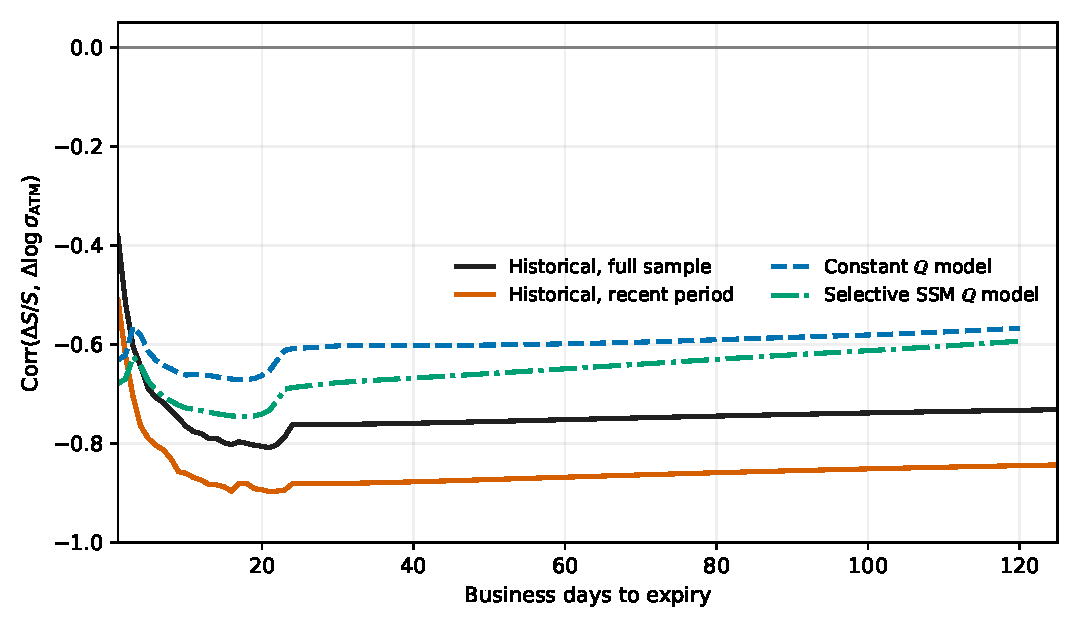
\includegraphics[width=0.88\textwidth]{atm_vol_spot_correlation_term_structure.pdf}
  \caption{Term structure of daily forward-adjusted spot-return correlation
  with changes in rolling-tenor ATM Black implied volatility.  Historical
  curves are measured under $\PP$; model curves are one-day conditional
  simulations under $\Q$ from the final calibration state.}
  \label{fig:spot-atm-volatility-correlation}
\end{figure}

\begin{table}[htbp]
  \centering
  \small
  \caption{Selected points from
  Figure~\ref{fig:spot-atm-volatility-correlation}.}
  \label{tab:spot-atm-volatility-correlation}
  \begin{tabular}{@{}rrrrr@{}}
    \toprule
    Business days
    & Historical
    & Recent
    & Constant $\Q$
    & Mamba SSM $\Q$ \\
    \midrule
      1 & $-0.382$ & $-0.510$ & $-0.632$ & $-0.679$ \\
      5 & $-0.689$ & $-0.790$ & $-0.614$ & $-0.674$ \\
     10 & $-0.766$ & $-0.861$ & $-0.662$ & $-0.729$ \\
     20 & $-0.806$ & $-0.894$ & $-0.663$ & $-0.741$ \\
     30 & $-0.762$ & $-0.881$ & $-0.603$ & $-0.678$ \\
     60 & $-0.752$ & $-0.869$ & $-0.599$ & $-0.650$ \\
     90 & $-0.742$ & $-0.856$ & $-0.586$ & $-0.621$ \\
    120 & $-0.733$ & $-0.845$ & $-0.568$ & $-0.594$ \\
    \bottomrule
  \end{tabular}
\end{table}

The selective backbone improves the root-mean-square discrepancy from the
full historical curve from $0.142$ to $0.098$.  It is close to the
full-sample 5D correlation ($-0.674$ versus $-0.689$), but does not reproduce
the stronger recent value of $-0.790$.  More generally, it is too negative
at 1--3D and too weak beyond roughly one month.  The corresponding discrepancy
from the recent curve is $0.185$, compared with $0.239$ for the constant
model.  Thus the selective state improves the observable leverage effect,
but the maturity shape and recent regime remain material targets for the
state-dependent correlation head in
Equation~\eqref{eq:conditional-spot-factor-correlation}.

\subsection{Portfolio-conditional entropic hedging}
\label{sec:portfolio-conditional-entropic-hedging}

Let $H$ be the remaining terminal liability of the current option portfolio,
$h$ the vector of current hedge holdings, $a$ the post-trade holdings, $R$
the future gains of the hedge instruments, and $C(a-h)$ the cost of changing
the hedge.  Conditional on the market state $X_t=x$, define the entropic risk
of a residual liability $Y$ by
\begin{equation}
  \rho_{\gamma,t}(Y)
  :=
  \frac{1}{\gamma}
  \log\E\!\left[\exp(\gamma Y)\mid X_t=x\right],
  \qquad \gamma>0.
  \label{eq:conditional-entropic-risk}
\end{equation}
The optimal one-period hedge is
\begin{equation}
  a^*_{\gamma,t}(H,h,x)
  :=
  \arg\min_a
  \rho_{\gamma,t}\!\left(H-a^\top R+C(a-h)\right).
  \label{eq:portfolio-entropic-hedge}
\end{equation}
Equation~\eqref{eq:portfolio-entropic-hedge} defines one hedge rule for
arbitrary portfolios, but not one portfolio-independent hedge position.  In
general, the rule must be conditioned on the remaining liability $H$.
Current cash wealth does not affect the optimizer because exponential utility
has constant absolute risk aversion.  Current risky holdings $h$ do matter in
the presence of transaction costs, position limits, or other trading
frictions.

Without trading costs, an interior optimizer satisfies
\begin{equation}
  \E\!\left[
    R\exp\!\left(\gamma(H-a^{*\top}R)\right)
    \mid X_t=x
  \right]
  =0.
  \label{eq:entropic-hedge-first-order-condition}
\end{equation}
The exponentially tilted measure in
Equation~\eqref{eq:entropic-hedge-first-order-condition} depends on $H$.
Consequently, hedges of two portfolios do not generally add, and changing
the portfolio notional changes the effective risk aversion.  In the
frictionless homogeneous case,
\begin{equation}
  a^*_{\gamma,t}(cH)=c\,a^*_{c\gamma,t}(H),
  \qquad c>0.
  \label{eq:entropic-notional-scaling}
\end{equation}
Thus claim size and risk aversion must be specified together in a hedging
benchmark.

There is a useful special case.  Suppose that $(H,R)$ is conditionally jointly
Gaussian, write $\mu_R:=\E[R\mid X_t=x]$, and let
$\Sigma_R:=\Var(R\mid X_t=x)$ be positive definite.  Then
\begin{equation}
  a^*_{\gamma,t}(H)
  =
  \Sigma_R^{-1}\operatorname{Cov}(R,H\mid X_t=x)
  +\frac{1}{\gamma}\Sigma_R^{-1}\mu_R.
  \label{eq:gaussian-entropic-hedge}
\end{equation}
The second term is the position that the optimizer would hold without the
liability.  Hence the incremental hedge is
\begin{equation}
  a^*_{\gamma,t}(H)-a^*_{\gamma,t}(0)
  =
  \Sigma_R^{-1}\operatorname{Cov}(R,H\mid X_t=x).
  \label{eq:gaussian-incremental-hedge}
\end{equation}
It is linear in $H$ and independent of $\gamma$.  Under $\Q$, where the
discounted gains have zero conditional mean, the zero-liability speculative
position vanishes.  Outside the Gaussian or complete-market setting,
Equations~\eqref{eq:gaussian-entropic-hedge} and
\eqref{eq:gaussian-incremental-hedge} no longer hold in general.

For GROMM, a universal hedging implementation should therefore learn or solve
the portfolio-conditioned policy
\begin{equation}
  \pi_\gamma\!\left(X_t,h_t,\Phi(H)\right),
  \label{eq:universal-portfolio-policy}
\end{equation}
where $\Phi(H)$ is a representation of the remaining portfolio.  A natural
choice is its vector of discounted payoffs on common GROMM scenarios,
possibly compressed into a payoff basis.  The reported hedge is the
incremental action
\begin{equation}
  \pi_\gamma\!\left(X_t,h_t,\Phi(H)\right)
  -
  \pi_\gamma\!\left(X_t,h_t,0\right).
  \label{eq:incremental-entropic-policy}
\end{equation}
This subtraction removes the speculative position under $\PP$ and should be
zero under $\Q$ in the absence of costs, constraints, and numerical error.

The ultimate performance statistic is the out-of-sample entropic risk of the
realized residual hedge loss.  For held-out episodes $p=1,\ldots,P$, with
residual losses $Y_p$, its empirical value is
\begin{equation}
  \widehat\rho_\gamma(Y)
  :=
  \frac{1}{\gamma}
  \log\left(
    \frac{1}{P}\sum_{p=1}^P \exp(\gamma Y_p)
  \right).
  \label{eq:empirical-entropic-hedging-risk}
\end{equation}
Comparisons should use identical market episodes, claim notionals, trading
costs, position limits, and risk-aversion levels.  Factor-law likelihood is a
useful dynamics diagnostic, but improvement in
Equation~\eqref{eq:empirical-entropic-hedging-risk} is the economically
relevant test.

\section{Acknowledgements}

We want to thank the team at Wharton for their WRDS \url{https://wrds-www.wharton.upenn.edu} portal and OptionMetrics \url{https://optionmetrics.com/united-states}
for providing their IvyDB data via this service. Without this data our work would not have been possible.


\appendix

\bibliographystyle{alpha}
\bibliography{refs}

\end{document}
